\documentclass{standalone}
\usepackage{tikz}
\usetikzlibrary{positioning}
\newdimen\nodeDist
\nodeDist=35mm
\begin{document}

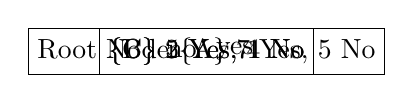
\begin{tikzpicture}[
    node/.style={%
      draw,
      rectangle,
    },
  ]

    \node [node] (A) {Root Node \{A\} 7 Yes, 5 No};
    \path (A) ++(-135:\nodeDist) node [node] (B) {\{B\} 2 Yes, 4 No};
    \path (A) ++(-45:\nodeDist) node [node] (C) {\{C\} 5 Yes, 1 No};

    \draw (A) -- (B) node [left,pos=0.25] {no}(A);
    \draw (A) -- (C) node [right,pos=0.25] {yes}(A);
\end{tikzpicture}

\end{document} 